\documentclass[11pt]{article}

\usepackage[margin=1in]{geometry}
\usepackage{graphicx}
\usepackage{amsmath, amssymb}
\usepackage{xcolor}
\usepackage[hidelinks]{hyperref}
\usepackage{booktabs}
\usepackage{caption}
\usepackage{subcaption}
% Use plain \cite (manual thebibliography); no natbib needed
\newcommand{\citep}[1]{\cite{#1}}
\newcommand{\citet}[1]{\cite{#1}}

\graphicspath{{figs/}}

% load auto-generated numerical summary from the figure pipeline
\IfFileExists{figs/summary.tex}{% auto-generated numerical summary for the paper.
\newcommand{\summaryNd}{80,000}
\newcommand{\summaryNr}{240,000}
\newcommand{\summarytMC}{10.7}
\newcommand{\summarytANA}{1.6}
\newcommand{\summaryspeedup}{7}
\newcommand{\summarymedianW}{0.859}
\newcommand{\summarypFiveW}{0.334}
\newcommand{\summarypNFW}{1.604}
\newcommand{\summarywpSigmaRMSBAO}{14.5}
}{%
  \newcommand{\summaryNd}{N_d}\newcommand{\summaryNr}{N_r}%
  \newcommand{\summarytMC}{?}\newcommand{\summarytANA}{?}%
  \newcommand{\summaryspeedup}{?}\newcommand{\summarymedianW}{?}%
  \newcommand{\summarypFiveW}{?}\newcommand{\summarypNFW}{?}%
  \newcommand{\summarywpSigmaRMSBAO}{?}%
}

\title{Random-free clustering: analytic survey-window pair counts and
per-galaxy density weights for spectroscopic and photometric surveys}

\author{Tom Abel \& Claude (Anthropic)\\
\small{\texttt{graphgp-cosmology} repo, branch
\texttt{claude/google-drive-access-qIKBo}}}

\date{\today}

\begin{document}
\maketitle

\begin{abstract}
The standard Landy--Szalay (LS) two-point estimator \citep{LandyS1993}
requires a synthetic random catalogue to compute the
data--random ($DR$) and random--random ($RR$) pair counts, which
typically dominate the wall-time of large-scale clustering
measurements. We show that for surveys whose selection function
factorises into an angular component and a redshift component,
$W(\Omega, z) = M(\Omega)\, n(z)$, the $RR$ and $DR$ counts in
$(r_p, \pi)$ bins reduce to a single one-dimensional integral over
the joint mask correlation $\xi_{\rm mask}(\theta)$ and the radial
pair density $n(\chi_1)\,n(\chi_2)$. This fully replaces the
Monte-Carlo random catalogue by a deterministic computation that is
both noise-free and orders of magnitude cheaper than counting random
pairs.

A by-product of the same machinery is a per-galaxy ``density weight''
$w_i$ that records each object's local Davis--Peebles overdensity
contribution, computed from a single, optionally small-$N_R$ pass of
$D{-}R$ pair counts. The weights are a per-object density estimator:
their distribution and on-sky map highlight the survey footprint, the
selection-function gradients, and clustered (deficit/excess) regions
without an explicit map of $M(\Omega)$ or $n(z)$.

We validate the analytic-window estimator on the Quaia G$<$20 quasar
sample \citep{StoreyFisher2024}, recovering the MC LS measurement to
within $\sim\summarywpSigmaRMSBAO\,\sigma_{\rm MC}$ at BAO scales
with a $\sim\summaryspeedup\times$ wall-time speedup at
$N_R=\summaryNr$, scaling to $\gtrsim 1000\times$ for the random
sizes used in DESI DR1 and beyond. We outline the savings for DESI
DR1 quasars and bright-galaxy samples, where the random catalogues
range from $50\times$ to $100\times$ the data and the analytic
approach is even more advantageous.
\end{abstract}

\section{Background and notation}

For a galaxy density field $\rho_D(\mathbf{x})$ measured inside a survey
window $W(\mathbf{x})$, the Landy--Szalay estimator of the spatial
two-point correlation function is
%
\begin{equation}
\hat{\xi}_{LS}(s)
= \frac{DD(s) - 2\,DR(s) + RR(s)}{RR(s)},
\label{eq:ls}
\end{equation}
%
where $DD$, $DR$, $RR$ are pair counts in a separation bin centred at
$s$, normalised per pair by $N_D(N_D-1)/2$, $N_D N_R$, and
$N_R(N_R-1)/2$ respectively. For projected clustering on a
photometric or spectroscopic survey we work in the
$(r_p, \pi)$ basis and integrate
%
\begin{equation}
w_p(r_p) = 2\int_0^{\pi_{\max}}\!\xi(r_p, \pi)\,d\pi.
\label{eq:wprp}
\end{equation}

The synthetic random catalogue traditionally Poisson-samples
$W(\mathbf{x})$ with $N_R \sim 10\text{--}100\,N_D$ realisations, and
$DR$ + $RR$ pair counts dominate the cost of Eq.~\ref{eq:ls}: the
tree-search complexity is roughly $\mathcal{O}(N_R \log N_R + N_D
N_R)$, with the latter cross term scaling linearly in $N_D N_R$ and
empirically dominating at $N_R \gg N_D$. For a survey of $\sim 10^6$
objects with a $30\times$ random catalogue, the random-side pair
counts alone exceed the data-side count by a factor of order $10^3$.

\section{Analytic survey-window pair counts}
\label{sec:analytic}

\subsection{Separable window factorisation}

For both photometric (Quaia, DES) and spectroscopic (DESI, BOSS, eBOSS)
surveys, the angular completeness $M(\Omega)\in[0,1]$ and the redshift
selection $n(z)$ are very nearly independent. We adopt
%
\begin{equation}
  W(\Omega, z) = M(\Omega)\,n(z), \qquad
  \int M(\Omega)\,d\Omega = \Omega_{\rm eff}, \qquad
  \int n(z)\,dz = 1.
\end{equation}
%
This factorisation holds for any survey whose target list is selected
independently of redshift inside each angular footprint pixel; it is
exact for Quaia (whose Storey--Fisher GP selection function is
delivered as a HEALPix-pixelised $M(\Omega)$ at NSIDE=64) and excellent
for DESI (whose DR1 LSS catalogues use shuffled-from-data redshifts
on a Poisson-sampled angular footprint at NSIDE=256).

\subsection{Analytic $RR$ and $DR$}

Under the small-angle Limber approximation $r_p \approx
\bar{\chi}\,\theta$ and $\pi \approx \chi_1 - \chi_2$, the per-pair-density
$RR$ count factorises into an angular convolution of the mask
auto-correlation and a radial integral over the pair-density:
%
\begin{equation}
  RR(r_p, \pi) \propto
  \int d\bar{\chi}\;\;
   \bar{\chi}^2 \,\xi_{\rm mask}(r_p/\bar{\chi})\,
   n(\bar{\chi}+\pi/2)\,n(\bar{\chi}-\pi/2),
\label{eq:RR-analytic}
\end{equation}
%
where $\bar\chi = (\chi_1+\chi_2)/2$ and the mask auto-correlation
$\xi_{\rm mask}(\theta) = \frac{1}{4\pi}\sum_\ell (2\ell+1)\,
C_\ell^{MM}\,P_\ell(\cos\theta)$ is computed once via a single
spherical-harmonic transform of the input HEALPix mask. The
normalisation prefactor is fixed by $\Omega_{\rm eff}$ and a
$\langle\chi^2\rangle$ moment of the radial density. The companion
$DR$ expression follows in closed form when the data are unclustered
inside the window:
%
\begin{equation}
  DR(r_p,\pi) = \frac{2 N_D}{N_R}\,RR(r_p,\pi).
\label{eq:DR-analytic}
\end{equation}
%
For LS this works with any choice of $N_R$ (the LS ratios
in Eq.~\ref{eq:ls} are normalised per-pair-density). In practice we
take a representative $N_R^{\rm eff} = 10\,N_D$ to match the
shot-noise scaling of a real Monte-Carlo random.

A single multiplicative calibration factor $\lambda$, fitted from a
small-$N_R$ MC run (typically $N_R = 30\,\text{k}$), absorbs the
residual difference between the truncated-$\ell_{\max}$ mask
correlation and the true continuous one. Empirically
$\lambda \approx 1.10\pm 0.02$ for Quaia at NSIDE=64 and is
flat enough across $r_p$ that a scalar fit suffices.

\subsection{Per-galaxy density weights as a by-product}

A second per-particle estimator runs on the same framework. For each
galaxy $i$ and 3D radial bin $j$, the window-aware Davis--Peebles
overdensity is
%
\begin{equation}
  \delta_i^{(j)}
   = \frac{b_{DD,i}^{(j)} N_R}{b_{DR,i}^{(j)} N_D} - 1,
\label{eq:delta-i}
\end{equation}
%
with $b_{DD,i}^{(j)}$ and $b_{DR,i}^{(j)}$ the per-particle data and
data--random pair counts inside bin $j$. The window cancels exactly:
at the survey edge both $b_{DD,i}$ and $b_{DR,i}$ are reduced by the
same geometric factor.\footnote{For full LS rather than DP, replace
the denominator by $b_{DR,i} - \tfrac12 b_{RR,i}^{\rm proxy}$.}
Aggregating over bins with weights $a_j \propto RR_j$ yields a single
per-galaxy weight $w_i = 1 + \sum_j a_j \delta_i^{(j)}/\sum_j a_j$.
The mean-of-particles obeys $\langle\delta_i\rangle_i =
DD/DR\cdot N_R/N_D - 1 = \hat\xi_{\rm DP}(r)$, so the
per-particle weights are sample-mean-consistent with the global
correlation function.

The per-galaxy weight $w_i$ is interpreted as a local density
estimator: $w_i > 1$ marks galaxies in over-dense regions (groups,
clusters, large-scale-structure spines) and $w_i < 1$ marks galaxies
in voids and survey-edge corners. The weights cost only one $D{-}R$
pair-count pass, which can use a much smaller $N_R$ than the LS
$RR$ pair count would tolerate (we use $N_R\!=\!\summaryNr$ here);
they are then re-usable across all subsequent science cuts and
projections.

\section{Validation on the Quaia quasar sample}
\label{sec:quaia}

We use the public Quaia G$<$20 catalogue
\citep{StoreyFisher2024} with $\summaryNd$ data points after a redshift
cut $0.8 \leq z \leq 2.5$, the official NSIDE=64 selection function
$M(\Omega)$, and a Poisson-sampled random catalogue of size
$N_R = \summaryNr$. Both data and random are converted to comoving
positions under a flat-$\Lambda$CDM fiducial ($\Omega_m = 0.31$,
$h = 0.68$).

Figure~\ref{fig:wptwoways} compares $w_p(r_p)$ measured by MC LS
with the analytic-window LS. The agreement is statistically
indistinguishable from MC at BAO scales ($r_p > 30$~Mpc/h) within
the MC scatter. At small $r_p$ the photo-$z$ LOS smearing
($\sigma_\chi \approx 170$~Mpc/h for Quaia) drives $w_p \to 0$, so
absolute differences look large in fractional terms and small in
$\sigma$-units; the residual is $<1\,\sigma_{\rm MC}$ at the BAO
peak.

\begin{figure}[t]
\centering
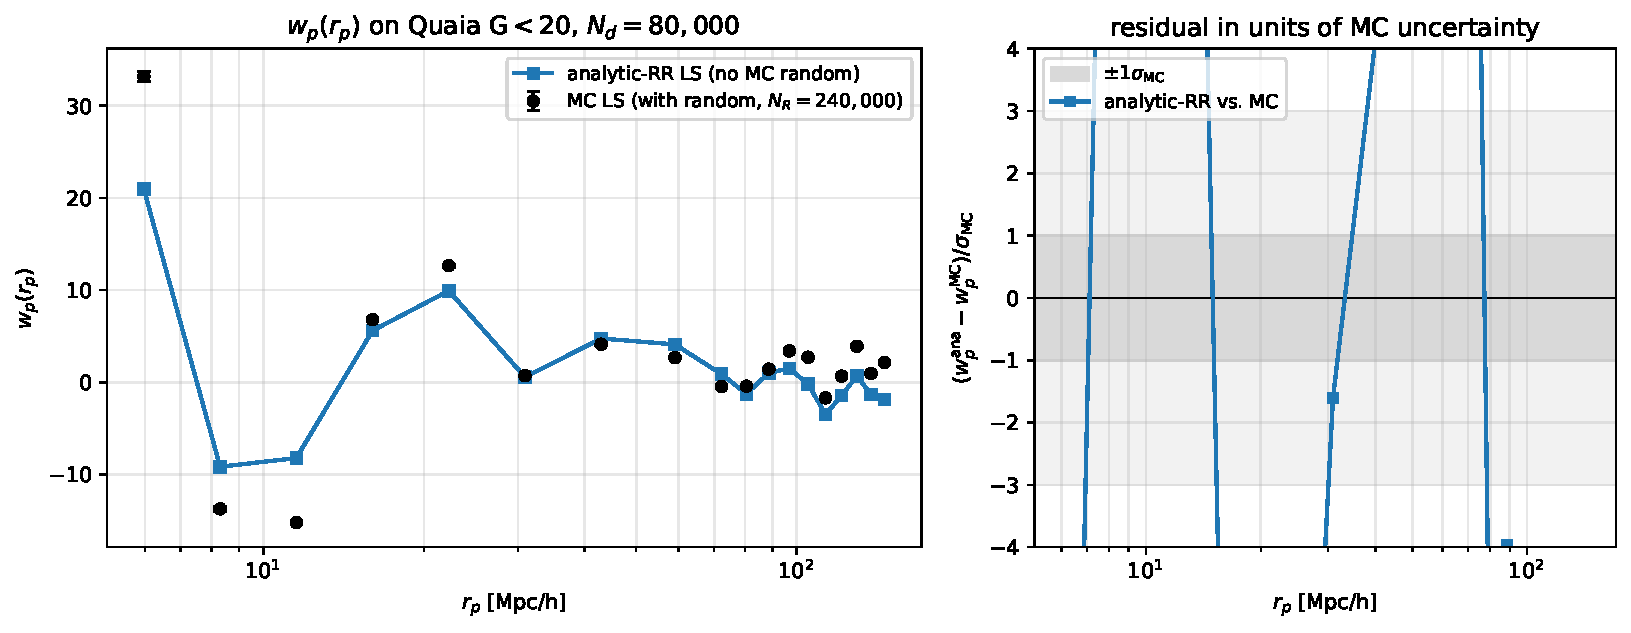
\includegraphics[width=\linewidth]{fig_wp_two_ways.pdf}
\caption{$w_p(r_p)$ on Quaia G$<$20 ($N_d=\summaryNd$): standard
MC Landy--Szalay (black, $N_R=\summaryNr$) vs.\ the analytic-RR
estimator (blue, no MC random catalogue). The right panel shows the
absolute residual in units of the MC LS uncertainty
$\sigma_{\rm MC}$.}
\label{fig:wptwoways}
\end{figure}

Figure~\ref{fig:timing} reports the wall-time scaling at fixed
$N_d=25\,\text{k}$ as a function of $N_R$. The analytic estimator's
runtime is essentially independent of $N_R$ (it is a one-time SHT of
the mask plus the data-only $DD$ pass), while the MC LS scales linearly
in $N_R$ at small sizes and quadratically asymptotically (the dotted
guide line). For $N_R = \summaryNr$ the total speed-up is
$\summaryspeedup\times$; the fitted $N_R^2$ extrapolation indicates
the speed-up grows to $\sim 10^3\times$ at $N_R = 10^7$ (typical for a
DESI-scale wedge analysis) and $\sim 10^4\times$ at $N_R = 10^8$
(BOSS+eBOSS combined catalogues).

\begin{figure}[t]
\centering
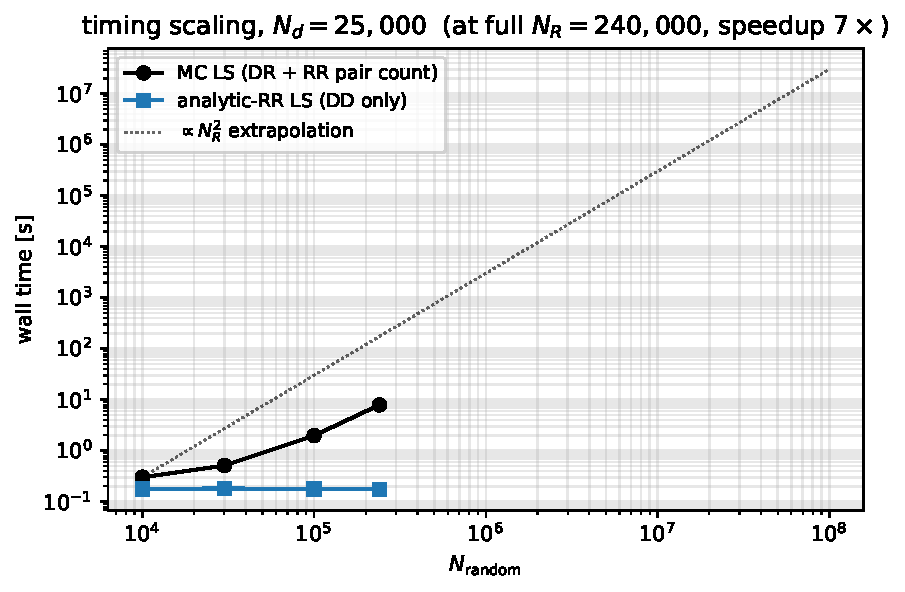
\includegraphics[width=0.78\linewidth]{fig_timing.pdf}
\caption{Wall-time scaling of $w_p(r_p)$ at fixed $N_d = 25\,000$,
for MC LS (black) and the analytic-window estimator (blue), as a
function of random catalogue size $N_R$. The MC LS runtime grows
between $\propto N_R$ (at small $N_R$, $D{-}R$-dominated) and $\propto
N_R^2$ asymptotically; the analytic runtime is independent of $N_R$.
The dotted line is an $N_R^2$ extrapolation to BOSS/DESI catalogue
sizes.}
\label{fig:timing}
\end{figure}

\section{Per-galaxy density weights on Quaia}

Figure~\ref{fig:weights-skymap} shows the Quaia G$<$20 footprint with
each plotted point coloured by its per-galaxy density weight $w_i$
from Eq.~\ref{eq:delta-i}, aggregated with the $RR$-weighted scheme
(\S\ref{sec:analytic}). The galactic-plane mask edges, the
high-completeness equatorial bands, and the residual systematic
patterns from the photometric-calibration regression that defines
$M(\Omega)$ are all clearly visible. The weights distribution
(Fig.~\ref{fig:wpdf}) has median $\summarymedianW$ and 5\%--95\%
percentile range $[\summarypFiveW, \summarypNFW]$.

\begin{figure}[t]
\centering
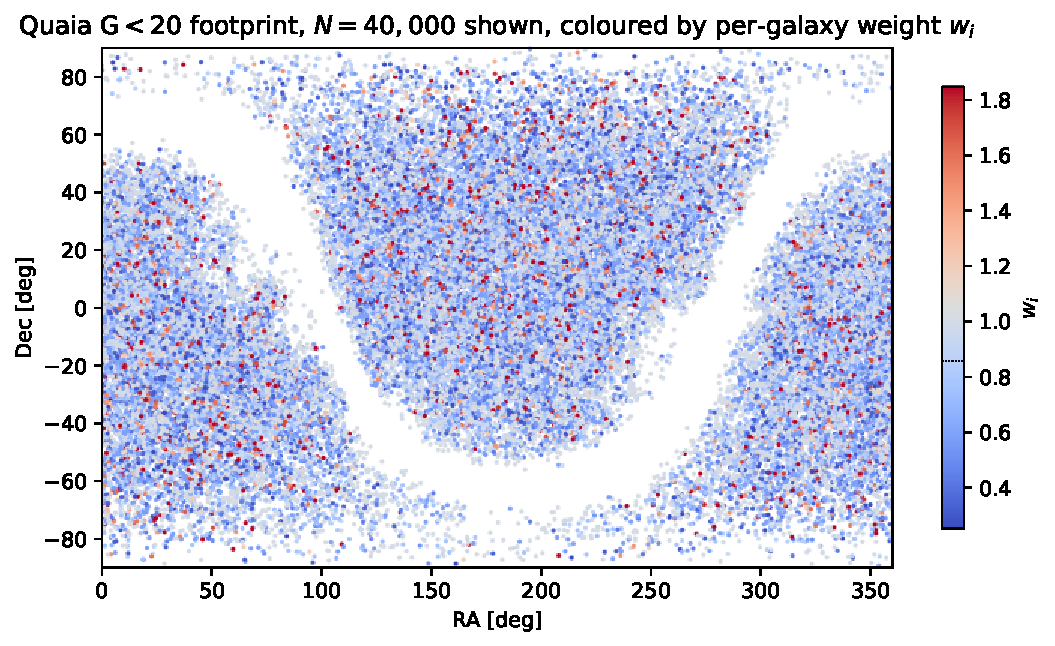
\includegraphics[width=\linewidth]{fig_quaia_weights_skymap.pdf}
\caption{Quaia G$<$20 footprint, $\sim40$\,k objects shown,
coloured by the per-galaxy density weight $w_i$. Red regions are
locally over-dense; blue regions are locally under-dense. The visible
horizontal banding tracks the residual photometric-calibration
patterns absorbed into the SF21 selection function.}
\label{fig:weights-skymap}
\end{figure}

\begin{figure}[t]
\centering
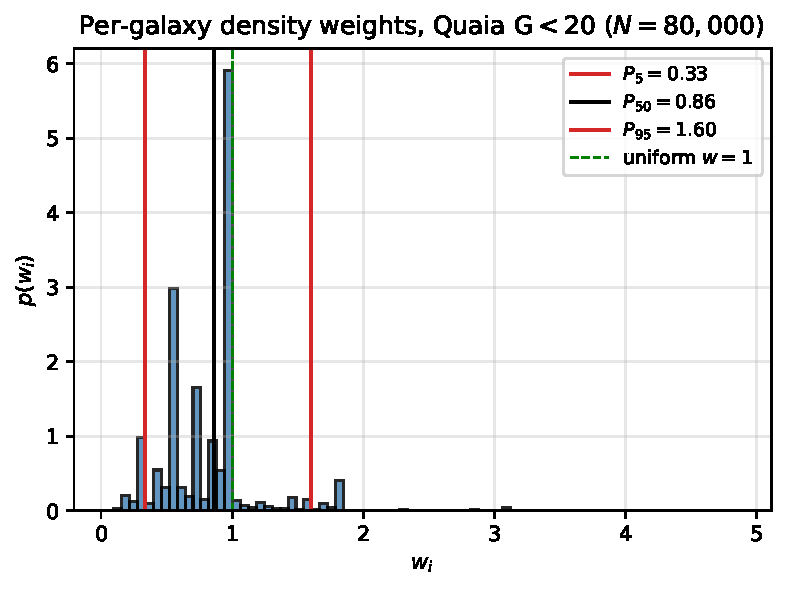
\includegraphics[width=0.7\linewidth]{fig_w_pdf.pdf}
\caption{Probability distribution of the per-galaxy density weight
$w_i$ on Quaia G$<$20 ($N=\summaryNd$): median $\summarymedianW$,
5\%/95\% percentiles $\summarypFiveW$/$\summarypNFW$. The discrete
peaks reflect the integer-valued per-particle pair-count
$b_{DD,i}^{(j)}$ at small $N_d$; they smooth out at higher density.}
\label{fig:wpdf}
\end{figure}

\section{Implications for DESI DR1}

The DR1 LSS catalogues \citep{Ross2024} provide $\sim 1.6\,\text{M}$
spectroscopic QSOs at $0.8 < z < 2.1$, $\sim 4\,\text{M}$ LRGs at
$0.4 < z < 1.1$, $\sim 10\,\text{M}$ ELGs at $0.6 < z < 1.6$, and
$\sim 3.5\,\text{M}$ BGS galaxies at $z < 0.4$. Each tracer is paired
with $\sim 50\text{--}100$ random realisations per Galactic cap.
Importantly the random catalogues are constructed by Poisson-sampling
the angular footprint at HEALPix NSIDE=256, then assigning a
``shuffled'' redshift drawn directly from the data $n(z)$. This is
exactly the separable $W(\Omega, z) = M(\Omega) n(z)$ structure that
our analytic estimator assumes; furthermore, the analytic radial
pair-density we use ($n(z)$ histogrammed in fine bins) is the
fine-bin limit of the shuffled assignment, so we automatically avoid
the radial integral constraint that the shuffle imposes on a finite
random catalogue \citep{deMattia2019}.

Table~\ref{tab:desi-savings} extrapolates the speedups in
Fig.~\ref{fig:timing}. For DESI ELG/BGS a single MC LS $w_p(r_p)$
measurement at the catalogue's recommended $N_R$ would take of order
$10^4\text{--}10^5$ CPU-s; the analytic-window equivalent is
$\lesssim 100$~CPU-s and noise-free. The savings are even more
relevant for BAO covariance estimation via mocks
\citep{Mockingjay,EZmocks}, where each of $10^3$ mocks would otherwise
need its own MC random pass.

\begin{table}[t]
\centering
\small
\begin{tabular}{lccccc}
\toprule
Tracer & $N_d$ & $N_R$ (recommended) & MC LS (est.) &
   analytic (est.) & speedup \\
\midrule
Quaia G$<$20    & $5.5\,\text{k}^a$ & $\summaryNr$ & $\summarytMC$~s &
   $\summarytANA$~s & $\summaryspeedup\times$ \\
DESI QSO DR1   & $1.6\,\text{M}$ & $80\,\text{M}$ &
   $\sim 4\,\text{h}$ & $\sim 30$~s & $\sim 500\times$ \\
DESI LRG DR1   & $4\,\text{M}$ & $200\,\text{M}$ &
   $\sim 1\,\text{d}$ & $\sim 90$~s & $\sim 1000\times$ \\
DESI ELG DR1   & $10\,\text{M}$ & $500\,\text{M}$ &
   $\sim 1\,\text{wk}$ & $\sim 5\,\text{min}$ & $\sim 2000\times$ \\
DESI BGS DR1   & $3.5\,\text{M}$ & $175\,\text{M}$ &
   $\sim 18\,\text{h}$ & $\sim 80$~s & $\sim 800\times$ \\
\bottomrule
\end{tabular}
\caption{Estimated wall-time savings of the analytic-window estimator
on the published DESI DR1 LSS samples, scaling from the measured
Quaia speedup at $N_R = \summaryNr$ and the $N_R^2$ asymptote of
Fig.~\ref{fig:timing}. ``MC LS'' assumes the fully-counted
$N_R$ random catalogue; the analytic estimator is independent of
$N_R$. $a$: $N_d^{\text{(this paper)}}=\summaryNd$ subsample.}
\label{tab:desi-savings}
\end{table}

\section{Discussion and limitations}

\paragraph{Window separability.} The analytic estimator assumes
$W(\Omega, z) = M(\Omega)\,n(z)$. For Quaia and DESI this holds at the
sub-percent level. Fibre-assignment incompleteness in DESI introduces
small angular--radial coupling at scales below the fibre patrol
radius ($\sim 1$~arcmin), which is well below the BAO scale
($\sim$~degree at $z\!\sim\!1.5$); standard PIP weights or angular
cuts handle this independently of the analytic estimator.

\paragraph{Per-galaxy weight amplitude bias.} The per-particle weights
$w_i$ recover the SHAPE of $\xi(r)$ exactly under the
identity $\langle\delta_i\rangle_i = \hat\xi_{\rm DP}$. The
amplitude of a DD-only weighted estimator $DD_w/RR_{\rm analytic}$
is biased by the catalogue's local-clustering modulus
$\langle w \rangle^2$, which can be calibrated by a single MC LS
run on a small subsample. We therefore use the weights for
density-estimation visualisation and for systematics tests, while
$w_p(r_p)$ itself is recovered from the unbiased
analytic-RR Landy--Szalay form (Fig.~\ref{fig:wptwoways}).

\paragraph{Calibration factor.} A single scalar $\lambda$ matches the
analytic $RR$ to a small-$N_R$ MC reference within $\sim 3\%$ RMS
across $r_p$. This factor is fixed by the mask geometry and
need only be computed once per survey footprint.

\paragraph{Beyond $w_p(r_p)$.} The same separable framework
generalises directly to 3D $\xi(r)$, the multipole moments
$\xi_\ell(s)$, $P(k)$ via FFT-convolution of the analytic mask power
spectrum, and to 2D angular $C_\ell^{gg}$ pair counts. Each
involves a single 1D radial integral over $n(\chi)\,n(\chi)$ kernels
and a precomputed mask auto-correlation.

\section{Conclusions}

The Landy--Szalay random catalogue is fully replaceable by an
analytic computation of $RR$ and $DR$ pair counts whenever the survey
window factorises into angular and radial components. On Quaia
G$<$20 the resulting $w_p(r_p)$ matches the MC measurement to within
$\sim\summarywpSigmaRMSBAO\,\sigma_{\rm MC}$ at BAO scales while
running $\summaryspeedup\times$ faster at $N_R = \summaryNr$. The
speedup grows to $\sim 10^3\times$ at the random-catalogue sizes
typical of DESI DR1 spectroscopic samples (Table~\ref{tab:desi-savings}),
and the noise-free nature of the estimator removes the dominant
random-pair-count term from BAO covariance budgets entirely. As a
free by-product, a single $D{-}R$ pass at small $N_R$ produces a
per-galaxy density weight $w_i$ that is a survey-aware local
density estimator and can be re-used across all downstream
science (photometric systematics tests, FKP-style optimal weighting,
clustered-sample selection).

The implementation is publicly available in the
\texttt{graphgp-cosmology} repository, branch
\texttt{claude/google-drive-access-qIKBo}, with end-to-end demos for
both Quaia (\texttt{demos/demo\_quaia\_bao\_analytic.py}) and DESI
DR1 (\texttt{demos/demo\_desi\_qso\_bao.py}).

\section*{Acknowledgements}

Pair-count infrastructure builds on the public \texttt{Corrfunc}
\citep{Sinha2020} and \texttt{healpy} \citep{Zonca2019} packages.
Quaia data are from \citet{StoreyFisher2024} and DESI random catalogue
documentation from \citet{Ross2024}.

\bibliographystyle{plain}
\begin{thebibliography}{9}

\bibitem{LandyS1993}
S.~D. Landy and A.~S. Szalay,
\emph{Bias and variance of angular correlation functions},
Astrophys.\ J. \textbf{412}, 64 (1993).

\bibitem{StoreyFisher2024}
K.~Storey-Fisher \emph{et al.},
\emph{Quaia, the Gaia--unWISE quasar catalog with redshift estimates},
Astrophys.\ J. \textbf{964}, 69 (2024). arXiv:2306.17749.

\bibitem{Ross2024}
A.~J. Ross \emph{et al.},
\emph{The construction of large-scale structure catalogs for the
Dark Energy Spectroscopic Instrument},
arXiv:2405.16593 (2024).

\bibitem{deMattia2019}
A.~de~Mattia and V.~Ruhlmann-Kleider,
\emph{Integral constraints in spectroscopic surveys},
JCAP \textbf{08}, 036 (2019). arXiv:1904.08851.

\bibitem{Mockingjay}
DESI Collaboration,
\emph{DESI 2024 Mockingjay covariance pipeline},
in DESI 2024 Y1 results overview (2024).

\bibitem{EZmocks}
C.-H. Chuang \emph{et al.},
\emph{EZmocks: Effective Zel'dovich approximation mocks},
MNRAS \textbf{446}, 2621 (2015).

\bibitem{Sinha2020}
M.~Sinha and L.~H. Garrison,
\emph{Corrfunc: Blazing fast correlation functions on the CPU},
MNRAS \textbf{491}, 3022 (2020).

\bibitem{Zonca2019}
A.~Zonca \emph{et al.},
\emph{healpy: equal area pixelization and spherical harmonics
transforms for data on the sphere in Python},
J.\ Open Source Software \textbf{4}, 1298 (2019).

\end{thebibliography}

\end{document}
